\documentclass[8pt, aspectratio=169]{beamer}

\usetheme{Copenhagen}

\setbeamercovered{transparent}

\usepackage{graphicx} % Required for inserting images
\usepackage[utf8]{inputenc}
\usepackage{tikz, pgfplots}
\pgfplotsset{compat=1.18}
\usetikzlibrary{positioning, arrows.meta}
\usetikzlibrary{bayesnet}
\usetikzlibrary[quotes]
\usetikzlibrary{arrows}
\usetikzlibrary{backgrounds}
\usetikzlibrary{shapes, shapes.geometric, shapes.misc}
\usepackage{tcolorbox}
\usepackage{glossaries}
% \usepackage{amsmath}
% \usepackage{amssymb}
\usepackage{amsthm}
% \usepackage{mathrsfs}
% \usepackage{array}
\usepackage{thmtools}
% \usepackage{bbm}

\usepackage[style=numeric,backend=biber]{biblatex}
\addbibresource{/home/benjamin/Folders_Python/MVA/MVA_Stage/LaTeX_rapport/citations_2.bib}
\addbibresource{/home/benjamin/Folders_Python/MVA/MVA_Stage/LaTeX_rapport/citations.bib}

\setbeamertemplate{navigation symbols}{}
\setbeamertemplate{footline}{%
  \leavevmode%
  \hbox{%
    \begin{beamercolorbox}[wd=.5\paperwidth,ht=2.25ex,dp=1ex,center]{author in head/foot}%
      \usebeamerfont{author in head/foot}%
      \insertframenumber{} / \inserttotalframenumber\hspace*{3em}\insertshortauthor
    \end{beamercolorbox}%
    \begin{beamercolorbox}[wd=.5\paperwidth,ht=2.25ex,dp=1ex,center]{title in head/foot}%
      \usebeamerfont{title in head/foot}\insertshorttitle
    \end{beamercolorbox}}%
  \vskip0pt%
}

\makeglossaries

\title{Dynamical Variational Autoencoders\\ Links to stochastic differential equations}

\author{
Benjamin Deporte : \href{mailto:benjamin.deporte@ens-paris-saclay.fr}{benjamin.deporte@ens-paris-saclay.fr}% student 1
}

% \text{ENS Paris-Saclay, MVA}

\date{August 2025 - DRAFT - Notes de Recherche}

\newacronym{dag}{DAG}{Directed Acyclic Graph}
\newacronym{vae}{VAE}{Variational Auto Encoder}
\newacronym{vlb}{VLB}{Variational Lower Bound}
\newacronym{elbo}{ELBO}{Evidence Lower Bound}
\newacronym{dvae}{DVAE}{Dynamical Variational Auto Encoder}
\newacronym{lstm}{LSTM}{Long Short Term Memory}
\newacronym{mlp}{MLP}{Multi Layer Perceptron}
\newacronym{vrnn}{VRNN}{Variational Recurrent Neural Network}
\newacronym{gpm}{GPM}{Graphical Probabilistic Model}
\newacronym{gpvae}{GP-VAE}{Gaussian Process Variational Auto Encoder}
\newacronym{gp}{GP}{Gaussian Process}
\newacronym{sde}{SDE}{Stochastic Differential Equation}
\newacronym{it}{IT}{Information Theory}
\newacronym{apen}{ApEn}{Approximate Entropy}
\newacronym{sampen}{SampEn}{Sample Entropy}
\newacronym{rts}{RTS}{Rauch-Tung-Striebel}
% conditional independence
\newcommand{\indep}{\perp \!\!\! \perp}
\newcommand{\notindep}{\not\!\perp\!\!\!\perp}
\newcommand{\cond}{\, \vert \,}
% real numbers
\newcommand{\R}{\mathbb{R}}
% expectation
\newcommand{\E}[1]{\mathbb{E}_{#1}}
% KL
\newcommand{\KL}[2]{\mathbb{KL}\left( #1 \vert\vert #2 \right)}
% VLB/ELBO
\newcommand{\VLB}{\mathcal{L}(\theta, \phi, X)}
% neural net Gaussian with diagonal covariance
\newcommand{\NNdiag}[3]{\mathcal{N}( #1 \vert #2, \text{diag}\, #3)}
% Brownian motion and related commands
\newcommand{\brownian}{(\Omega, \mathcal{F}, (\mathcal{F}_t)_{t \geq 0}, (B_t)_{t \geq 0}, \mathbb{P})}
\newcommand{\filtration}{(\mathcal{F}_t)_{t \in T}}
\newcommand{\espaceprob}{(\Omega, \mathcal{F}, \mathbb{P})}
\newcommand{\lunomega}{L^1(\Omega, \mathcal{F}, \mathbb{P})}
\newcommand{\ldeuxomega}{L^2(\Omega, \mathcal{F}, \mathbb{P})}
\newcommand{\norm}[1]{\vert \vert #1 \vert \vert}

\begin{document}

\maketitle

\begin{frame}{Summary}
    \tableofcontents
\end{frame}

\section{Abstract}\label{Abstract}

\begin{frame}{Abstract}
    \begin{itemize}
        \item <1-> \textbf{\glspl{vae}} have limitations when dealing with data sequences, due to i.i.d assumption.
        \item <2-> \textbf{Dynamical Variational Auto Encoders} (\cite{girin_dynamical_2022}) are adapted to data sequences
            \begin{itemize}
                \item Temporal dependency built into latent prior
                \item Discrete or continuous time prior
                \item Observation model as in regular \glspl{vae}: Gaussian, Bernoulli, Student-t...
            \end{itemize}
        \item <3-> \textbf{Link to Stochastic Calculus}
            \begin{itemize}
                \item Solutions to linear \glspl{sde} are Gaussian processes : run prior \gls{gp} regression at linear cost.
                \item Solutions to general \glspl{sde} are Markov processes : link to more general \glspl{latent sde}
            \end{itemize}
        \item <4-> \textbf{What we will cover today}
            \begin{itemize}
                \item General theory of \glspl{dvae}
                \item Review of some discrete and continuous time \glspl{dvae} with XPs : \gls{dkf}, \gls{vrnn}, \gls{gpvae}
                \item Stochastic calculus survival kit
                \item Relationships between \glspl{dvae} and stochastic calculus
                \item Early perspective on \glspl{latent ode} and \glspl{latent sde}
            \end{itemize}
    \end{itemize}
\end{frame}

\section{Dynamical Variational AutoEncoders}\label{DVAEs}

\begin{frame}{Dynamical Variational Auto Encoders : what is it ?}
    \begin{itemize}
        \item <1-> \textbf{Dynamical Variational Auto Encoders} are a class of VAEs in which some structure is given to the latent variables to encode the time dependency.
        \item <2-> DVAEs can be discrete-time or continuous models, can require regularly-sampled data, or can manage irregularly sampled data.
        \item <3-> For example, a Kalman filter is the simplest DVAE : 
        \begin{itemize}
            \item first order Markov chain for latent variables
            \item linear Gaussian observation model.
        \end{itemize}
        \item <4-> As in vanilla VAEs, inference is performed by evidence lower bound maximization.
        \item <5-> Notations
            \begin{tcolorbox}[colback=blue!5!white,colframe=black!75!black]
                \begin{itemize}
                    \item the data is a sequence of $T$ points noted \textbf{$x_{1:T}$} $= \{(x_t)_{t=1,...,T}\} \in \mathbb{R}^F$.
                    \item the sequence of the associated $T$ latent variables is \textbf{$z_{1:T}$} $= \{(z_t)_{t=1,...,T}\} \in \mathbb{R}^L$
                    \item optionally, there may be a sequence of -usually deterministic- $T$ inputs $u_{1:T} = \{(u_t)_{t=1,...,T}\} \in \mathbb{R}^U$
                \end{itemize}
            \end{tcolorbox}
    \end{itemize}
\end{frame}

\begin{frame}{General formulation of DVAE}
    \begin{block}{Generative model}
        \begin{align*}
            p(x_{1:T}, z_{1:T} \vert u_{1:T}) &= \prod_{t=1}^T p(x_t, z_t \vert x_{1:t-1}, z_{1:t-1}, u_{1:T}) \\
            &= \prod_{t=1}^T p(x_t \vert x_{1:t-1}, z_{1:t}, u_{1:T}) p(z_t \vert x_{1:t-1}, z_{1:t-1}, u_{1:T}) \\
            &= \prod_{t=1}^T p(x_t \vert x_{1:t-1}, z_{1:t}, u_{1:t}) p(z_t \vert x_{1:t-1}, z_{1:t-1}, u_{1:t})
        \end{align*}
    \end{block}
    The only assumption that is made is a a causal dependency of the $x_t, z_t$ on the inputs $u_{1:t}$, thus allowing to change the conditioning $\vert u_{1:T}$ into $\vert u_{1:t}$.

    In the rest of the presentation, we will consider systems with no input, and drop the conditioning on $u_{1:t}$ to simplify notations. However, the reasoning remains the same with inputs.
\end{frame}

\begin{frame}{Posteriors}
    \begin{itemize}
        \item <1-> The true posterior  $p(z_{1:T} \vert x_{1:T})$ is usually untractable, but can be developed:
            \begin{align*}
                p(z_{1:T} \vert x_{1:T}) &= \prod_{t=1}^T p(z_t \vert z_{1:t-1}, x_{1:T})
            \end{align*}
        % It can be noted that the true posterior exhibits a dependence of $z_t$ on \textit{past} $z_{1:t-1}$, but a dependence on the \textit{whole} data sequence $x_{1:T}$ (think Kalman smoother).
        \item <2-> As in vanilla \glspl{vae}, the inference model is the approximation of the true posterior by an parametric encoder $q_{\phi}(z_{1:T} \vert x_{1:T})$, where $\phi$ is the set of parameters:
            \begin{align*}
                q_{\phi}(z_{1:T} \vert x_{1:T}) &= \prod_{t=1}^T q_\phi(z_t \vert z_{1:t-1}, x_{1:T})
            \end{align*}
        \item <3-> Depending on the chosen graphical models and the corresponding D-separation results, the observation model $p_{\theta_x}(x_t \vert x_{1:t-1}, z_{1:t}, u_{1:t})$ (with $\theta_x$ the set of parameters of the observation model) and approximate posterior $q_\phi(z_t \vert z_{1:t-1}, x_{1:T})$ will simplify. 
        \item <4-> It is also considered a good practice to copy the expression of $q_\phi(z_t \vert z_{1:t-1}, x_{1:T})$ from the expression of the true posterior resulting from the D-separation analysis (see next chapters for examples).
    \end{itemize}
\end{frame}

\begin{frame}{Likelihood}
    \begin{itemize}
        \item <1-> Observation model and encoder:
        \begin{align}
            p_{\theta}(x_{1:T}, z_{1:T}) &= \prod_{t=1}^T p_{\theta_x}(x_t \vert x_{1:t-1}, z_{1:t}) p_{\theta_z}(z_t \vert z_{1:t-1}, x_{1:t-1}) \\
            \label{q_phi_dev}
            q_\phi(z_{1:T} \vert x_{1:T}) &= \prod_{t=1}^T q_\phi (z_t \vert z_{1:t-1}, x_{1:T})
        \end{align}
        \item <2-> Log likelihood
        \begin{align}
            \log{p(x_{1:T})} &= \log{\frac{p(x_{1:T}, z_{1:T})}{p(z_{1:T} \vert x_{1:T})}} \\
            &= \E{q_{\phi}(z_{1:T}\vert x_{1:T})} \log{\frac{p(x_{1:T}, z_{1:T})}{q_{\phi}(z_{1:T}\vert x_{1:T})} \frac{q_{\phi}(z_{1:T}\vert x_{1:T})}{p(z_{1:T} \vert x_{1:T})}} \\
            &= \E{q_{\phi}(z_{1:T}\vert x_{1:T})} \log{\frac{p(x_{1:T}, z_{1:T})}{q_{\phi}(z_{1:T}\vert x_{1:T})} + \KL{q_{\phi}(z_{1:T}\vert x_{1:T})}{p(z_{1:T} \vert x_{1:T})}} \\
            &\geq \E{q_{\phi}(z_{1:T}\vert x_{1:T})} \log{\frac{p(x_{1:T}, z_{1:T})}{q_{\phi}(z_{1:T}\vert x_{1:T})}} = \VLB
        \end{align}
    \end{itemize}
\end{frame}

\begin{frame}{Variational Lower Bound}
    \begin{itemize}
        \item Lower bound:
        \begin{align}
            \VLB &= \E{q_{\phi}(z_{1:T}\vert x_{1:T})} \log{\left( \frac{\prod_{t=1}^T p_{\theta_x}(x_t \vert x_{1:t-1}, z_{1:t}) p_{\theta_z}(z_t \vert z_{1:t-1}, x_{1:t-1})}{\prod_{t=1}^T q_\phi (z_t \vert z_{1:t-1}, x_{1:T})} \right)} \\
            &= \E{q_{\phi}(z_{1:T}\vert x_{1:T})} \left(  \sum_{t=1}^T \log{p_{\theta_x}(x_t \vert x_{1:t-1}, z_{1:t})} - \sum_{t=1}^T \log{\frac{q_\phi (z_t \vert z_{1:t-1}, x_{1:T})}{p_{\theta_z}(z_t \vert z_{1:t-1}, x_{1:t-1})}}
            \right) \\
            &= \sum_{t=1}^T \E{q_\phi(z_{1:t} \vert x_{1:T})} \log{p_{\theta_x}(x_t \vert x_{1:t-1}, z_{1:t})} -\\
            &\sum_{t=1}^T \E{q_\phi(z_{1:t-1} \vert x_{1:T})} \KL{q_\phi(z_t \vert z_{1:t-1}, x_{1:T})}{p_{\theta_z}(z_t \vert z_{1:t-1}, x_{1:t-1})}
        \end{align}
        \item The first term is the usual \textbf{reconstruction error}.
        \item The second term is a regularization term, summing over the time steps the average divergence between the approximate posterior distribution of the latent variable at time $t$, and its real distribution.
        \item As in vanilla \gls{vae}, the sampling over $q_\phi$ requires the use of the "re parametrization trick" (see \cite{kingma_introduction_2019}), for $\VLB$ to be differentiable w.r.t. $\theta, \phi$.
    \end{itemize}
\end{frame}

\begin{frame}{Summary DVAE}
    \begin{tcolorbox}[colback=blue!5!white,colframe=black!75!black,title=General Dynamical VAEs : generative and inference models; variational lower bound]
        % \begin{itemize}
            % \item \textbf{generative and inference model}s
            \begin{align}
                \label{gen_model_dvae}
                p(x_{1:T}, z_{1:T}) &= \prod_{t=1}^T p_{\theta_x} (x_t \vert x_{1:t-1}, z_{1:t}) p_{\theta_z}(z_t \vert z_{1:t-1}, x_{1:t-1}) \\
            % \end{align}
            % \item \textbf{inference model}
            % \begin{align}
                \label{inf_model_dvae}
                q_{\phi}(z_{1:T} \vert x_{1:T}) &= \prod_{t=1}^T q_\phi(z_t \vert z_{1:t-1}, x_{1:T}) \\
            % \end{align}
            % % \item \textbf{\gls{vlb} for training}
            % \begin{align}
                \label{vlb_dvae}
                \begin{split}
                 \VLB &= \sum_{t=1}^T \E{q_\phi(z_{1:t} \vert x_{1:T})} \log{p_{\theta_x}(x_t \vert x_{1:t-1}, z_{1:t})} \\ &- \sum_{t=1}^T \E{q_\phi(z_{1:t-1} \vert x_{1:T})} \KL{q_\phi(z_t \vert z_{1:t-1}, x_{1:T})}{p_{\theta_z}(z_t \vert z_{1:t-1}, x_{1:t-1})}
                 \end{split}
            \end{align}
        % \end{itemize}
    \end{tcolorbox}
\end{frame}

%
%
% ==========================================================
%
% === DEEP KALMAN FILTER ===
%
% ==========================================================
%
%

\begin{frame}{Deep Kalman Filter}
Deep Kalman Filter \gls{dag}:

\begin{figure}[h]
        \centering
        % \includegraphics[width=0.5\linewidth]{}
        \label{fig:graphical_model_dkf}
    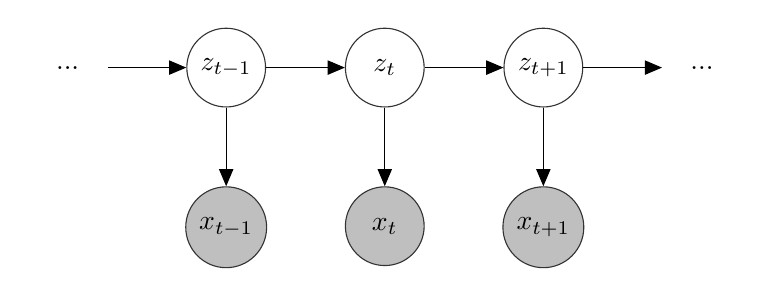
\begin{tikzpicture}[
        HIDDEN/.style={circle, draw=black!0, thin, minimum size=10mm},
        UNOBS/.style={circle, draw=black!80, thin, minimum size=10mm},
        OBS/.style={circle, draw=black!80, fill=gray!50, thin, minimum size=10mm}
    ]
    % nodes
    \node[HIDDEN] (a) {$...$};
    \node[UNOBS] (z_t_1) [right= of a] {$z_{t-1}$} edge[<-, thin] (a);
    \node[UNOBS] (z_t)  [right= of z_t_1] {$z_{t}$} edge[<-, thin] (z_t_1);
    \node[UNOBS] (z_t_p1) [right= of z_t] {$z_{t+1}$} edge[<-, thin] (z_t);
    \node[HIDDEN] (e) [right= of z_t_p1] {$...$} edge[<-, thin] (z_t_p1);
    \node[OBS] (x_t_1) [below= of z_t_1] {$x_{t-1}$} edge[<-, thin] (z_t_1);
    \node[OBS] (x_t) [below= of z_t] {$x_{t}$} edge[<-, thin] (z_t);
    \node[OBS] (x_t_p1) [below= of z_t_p1] {$x_{t+1}$} edge[<-, thin] (z_t_p1);
    \end{tikzpicture}
    \caption{Probabilistic model of a Deep Kalman Filter}
\end{figure}
\end{frame}

\begin{frame}{Deep Kalman Filter - generative model}
Using \textbf{D-separation} on the \gls{dag} to simplify the general \gls{dvae} expressions \ref{gen_model_dvae} and \ref{inf_model_dvae}. Conditioning on $z_t$ and $z_{t-1}$ drives:
\begin{align}
    p_{\theta_x}(x_t \vert x_{1:t-1}, z_{1:t}) &= p_{\theta_x}(x_t \vert z_t) \\
    p_{\theta_z}(z_t \vert z_{1:t-1}, x_{1:t}) &= p_{\theta_z}(z_t \vert z_{t-1}) \\
    \label{dkf_posterior}
    q_{\phi}(z_t \vert z_{1:t-1}, x_{1:T}) &= q_{\phi}(z_t \vert z_{t-1}, x_{t:T}) 
\end{align}
\end{frame}

\begin{frame}{Deep Kalman Filter - generative model - 2}
We then choose Gaussian distributions for $p_{\theta_x}, p_{\theta_z}$ and $q_\phi$, with mean and diagonal covariance, learnt by neural networks.
\begin{align}
    p_{\theta_x}(x_t \vert z_t) &= \NNdiag{x_t}{\mu_{\theta_x}(z_t)}{\sigma_{\theta_x}^2(z_t)}\\
    p_{\theta_z}(z_t \vert z_{t-1}) &= \NNdiag{z_t}{\mu_{\theta_z}(z_{t-1})}{\sigma_{\theta_z}^2(z_{t-1})}\\
    q_{\phi}(z_t \vert z_{t-1}, x_{t:T}) &= \NNdiag{z_t}{\mu_{\phi}(z_{t-1}, x_{t:T})}{\sigma_{\theta_z}^2(z_{t-1},x_{t:T})}
\end{align}
Some other formulations of the approximate posterior (encoder) are possible. For example:
\begin{align*}
    q_{\phi}(z_t \vert z_{t-1}, x_t) \\
    q_{\phi}(z_t \vert z_{1:t}, x_{1:t}) \\
    q_{\phi}(z_t \vert z_{1:T}, x_{1:T})
\end{align*}
We have chosen \ref{dkf_posterior} for the implementation, as it has the same formulation as the true posterior and respects the corresponding dependencies.
\end{frame}

\begin{frame}{Deep Kalman Filter - ELBO}
% \begin{align*}
%     q_{\phi}(z_{1:t} \vert x_{1:T}) = q_{\phi}(z_{1:t-1} \vert z_t, x_{1:T}) q_{\phi}(z_t \vert x_{1:T})
% \end{align*}
Using D-Separation, the \gls{elbo} \ref{vlb_dvae} simplifies into:
\begin{align}
    \VLB &= \sum_{t=1}^T \E{q_\phi(z_{1:t} \vert x_{1:T})} \log{p_{\theta_x}(x_t \vert z_t)} - \sum_{t=1}^T \E{q_\phi(z_{1:t-1} \vert x_{1:T})} \KL{q_{\phi}(z_t \vert z_{t-1}, x_{t:T})}{p_{\theta_z}(z_t \vert z_{t-1})} \\
    &= \sum_{t=1}^T \E{q_\phi(z_{t} \vert x_{1:T})} \log{p_{\theta_x}(x_t \vert z_t)} - \sum_{t=1}^T \E{q_\phi(z_{t-1} \vert x_{1:T})} \KL{q_{\phi}(z_t \vert z_{t-1}, x_{t:T})}{p_{\theta_z}(z_t \vert z_{t-1})}
\end{align}
\end{frame}

\begin{frame}{Deep Kalman Filter - summary}
\begin{tcolorbox}[colback=blue!5!white,colframe=black!75!black,title=Deep Kalman Filter]
\begin{itemize}
    \item \textbf{generative model}
    \begin{align}
        \label{gen_model_dkf}
        p_{\theta_x}(x_t \vert z_t) &= \NNdiag{x_t}{\mu_{\theta_x}(z_t)}{\sigma_{\theta_x}^2(z_t)}\\
        p_{\theta_z}(z_t \vert z_{t-1}) &= \NNdiag{z_t}{\mu_{\theta_z}(z_{t-1})}{\sigma_{\theta_z}^2(z_{t-1})}
    \end{align}
    \item \textbf{inference model}
    \begin{align}
        \label{inf_model_dkf}
        q_{\phi}(z_t \vert z_{t-1}, x_{t:T}) &= \NNdiag{z_t}{\mu_{\phi}(z_{t-1}, x_{t:T})}{\sigma_{\theta_z}^2(z_{t-1},x_{t:T})}
    \end{align}
    \item \textbf{\gls{vlb} for training}
    \begin{align}
        \label{vlb_dkf}
        \VLB &= \sum_{t=1}^T \E{q_\phi(z_{t} \vert x_{1:T})} \log{p_{\theta_x}(x_t \vert z_t)} - \sum_{t=1}^T \E{q_\phi(z_{t-1} \vert x_{1:T})} \KL{q_{\phi}(z_t \vert z_{t-1}, x_{t:T})}{p_{\theta_z}(z_t \vert z_{t-1})}
    \end{align}
\end{itemize}
\end{tcolorbox}
\end{frame}

\begin{frame}{DKF - Torch}
    \begin{itemize}
        \item The $\KL{q_\phi}{p_{\theta_z}}$'s have a close form, as the two distributions are Gaussians (see \ref{sec:KL-two-exponential-family-distributions})

        \item Following \cite{girin_dynamical_2022}, we use forward \gls{lstm} to encode sequences such as $x_{1:t}$, and backward \gls{lstm} to encode sequences such as $x_{t:T}$, as inputs into the \gls{mlp} parametrizing the distributions. 
        \item For example:
            \begin{align*}
                \overleftarrow{g_t} &= \text{Backward LSTM}(\overleftarrow{g_{t+1}}, x_t) \,\, (\text{encodes} \,\, x_{t:T}) \\
                q_{\phi}(z_t \vert z_{t-1}, x_{t:T}) &= \NNdiag{z_t}{\mu_{\phi}(z_{t-1}, \overleftarrow{g_t})}{\sigma_{\phi}^2(z_{t-1}, \overleftarrow{g_t})}
            \end{align*}
    \end{itemize}
\end{frame}


\begin{frame}[fragile]{DKF - Torch - Schematic blocks}
The PyTorch implementation is described below:
%
%
%------- DEEP KALMAN FILTER ------------------------------
%
%
% % \begin{landscape}
\begin{figure}[h]
    \centering
% % \begin{centering}
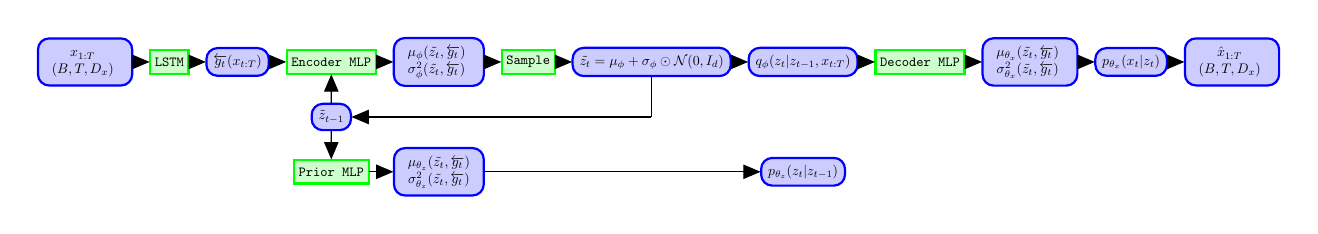
\begin{tikzpicture}[
    scale=0.70,
    every node/.style={scale=0.50},
    torch/.style={
        rectangle, 
        minimum size=6mm, 
        thick, 
        draw=green!100, 
        fill=green!20, 
        font=\ttfamily
        },
    math/.style={
        rectangle, 
        % minimum height=1cm,
        % minimum width=2cm,
        rounded corners, 
        thick, 
        draw=blue!100,
        fill=blue!20,
        align=center,
        anchor=center,
        inner sep=5pt
        },
    point/.style={
        circle,
        inner sep=0pt,
        minimum size=0pt,
        }
    ]
% \matrix[row sep = 1mm, column sep=5mm]{}
\matrix[row sep = 2mm, column sep=2mm]{
% first row
\node[math] (xt) {
    $\begin{array}{c}
            x_{1:T} \\
            (B,T,D_x)
    \end{array}$
}; &
\node[torch] (lstm) {LSTM}; & 
\node[math] (gt) {$\overleftarrow{g_t}(x_{t:T})$}; &
\node[torch] (enco) {Encoder MLP}; &
\node[math] (phi) {
    $\begin{array}{c}
            \mu_{\phi}(\tilde{z_t}, \overleftarrow{g_t}) \\
            \sigma_{\phi}^2(\tilde{z_t}, \overleftarrow{g_t})
    \end{array}$
}; &
\node[torch] (sample) {Sample}; &
\node[math] (z_tilde) {$\tilde{z_t}= \mu_{\phi} + \sigma_{\phi} \odot \mathcal{N}(0, I_d)$}; & 
\node[math] (q_phi) {$q_{\phi}(z_t \vert z_{t-1}, x_{t:T})$}; &
\node[torch] (deco) {Decoder MLP}; &
\node[math] (theta_x) {
    $\begin{array}{c}
        \mu_{\theta_x}(\tilde{z_t}, \overleftarrow{g_t}) \\
        \sigma_{\theta_x}^2(\tilde{z_t}, \overleftarrow{g_t})
    \end{array}$
}; &
\node[math] (p_theta_x) {$p_{\theta_x}(x_t \vert z_t)$}; &
\node[math] (x_hat) {
    $\begin{array}{c}
            \hat{x}_{1:T} \\
            (B,T,D_x)
    \end{array}$
}; \\
%second row
& & & \node[math] (z_t_1) (z_t_1) {$\tilde{z}_{t-1}$}; & & & \node[point] (coin) {}; & & &; \\
%third row
& & & \node[torch] (prior) {Prior MLP}; &
\node[math] (theta_z) {
    $\begin{array}{c}
            \mu_{\theta_z}(\tilde{z_t}, \overleftarrow{g_t}) \\
            \sigma_{\theta_z}^2(\tilde{z_t}, \overleftarrow{g_t})
    \end{array}$}; & & &
\node[math] (p_theta_z) {$p_{\theta_z}(z_t \vert z_{t-1})$}; &
& &; \\
};
\path   (xt) edge [->, thin] (lstm)
        (lstm) edge [->, thin] (gt)
        (gt) edge [->, thin] (enco)
        (enco) edge [->, thin] (phi)
        (phi) edge [->, thin] (sample)
        (sample) edge [->, thin] (z_tilde)
        (z_tilde) edge [->, thin] (q_phi)
        (q_phi) edge[->, thin] (deco)
        (deco) edge [->, thin] (theta_x)
        (theta_x) edge [->, thin] (p_theta_x)
        (p_theta_x) edge [->, thin] (x_hat)
        (z_t_1) edge [->, thin] (enco)
        (prior) edge [<-, thin] (z_t_1)
        (theta_z) edge [<-, thin] (prior)
        (theta_z) edge[->, thin] (p_theta_z)
        (z_tilde) edge [-, thin] (coin)
        (coin) edge [->, thin] (z_t_1);
\end{tikzpicture}
% --- Loss DKF
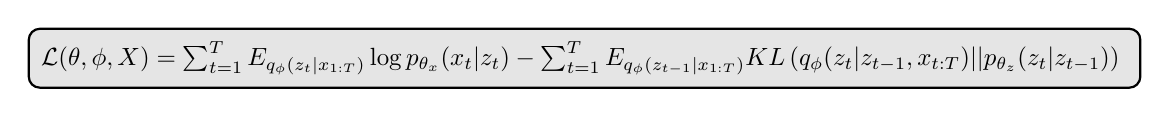
\begin{tikzpicture}[
    scale=0.90,
    every node/.style={scale=0.90},
    math/.style={
        rectangle, 
        % minimum height=1cm,
        % minimum width=2cm,
        rounded corners, 
        thick, 
        draw=black!100,
        fill=gray!20,
        align=center,
        anchor=center,
        inner sep=5pt
        },
    ]
    \node[math] {
            $\VLB = \sum_{t=1}^T \E{q_\phi(z_{t} \vert x_{1:T})} \log{p_{\theta_x}(x_t \vert z_t)} - \sum_{t=1}^T \E{q_\phi(z_{t-1} \vert x_{1:T})} \KL{q_{\phi}(z_t \vert z_{t-1}, x_{t:T})}{p_{\theta_z}(z_t \vert z_{t-1})}$
    };
\end{tikzpicture}
% % \end{centering}
% % \caption{Deep Kalman Filter Model Architecture}
\end{figure}
% % \end{landscape}
\end{frame}

%
%
% ==========================================================
%
% === VARIATIONAL RNN ===
%
% ==========================================================
%
%

\begin{frame}{Variational RNN}
The \gls{vrnn} is the most expressive \gls{dvae}, in that sense that the general expressions \ref{gen_model_dvae}, \ref{inf_model_dvae} and \gls{vlb} \ref{vlb_dvae} can not be simplified.

The \gls{gpm} of the \gls{vrnn} assumes full connections between latent variables, and between observed variables, to account for the full unsimplified expressions. Specifically:

\begin{figure}[h]
    \centering
    % \includegraphics[width=0.5\linewidth]{}
    \label{fig:graphical_model_vrnn}
\begin{tikzpicture}[
    HIDDEN/.style={circle, draw=black!0, thin, minimum size=10mm},
    UNOBS/.style={circle, draw=black!80, thin, minimum size=10mm},
    OBS/.style={circle, draw=black!80, fill=gray!50, thin, minimum size=10mm}
]
% nodes
\node[HIDDEN] (zs) {$...$}; % start z
\node[HIDDEN] (xs) [below= of zs] {$...$}; % start x
\node[UNOBS] (z_t_1) [right= of zs] {$z_{t-1}$} edge[<-, thin] (a);
\node[OBS] (x_t_1) [below= of z_t_1] {$x_{t-1}$}    edge[<-, thin] (z_t_1)
                                                    edge[<-, thin] (xs);
\node[UNOBS] (z_t)  [right= of z_t_1] {$z_{t}$} edge[<-, thin] (z_t_1)
                                                edge[<-, thin] (x_t_1);
\node[OBS] (x_t) [below= of z_t] {$x_{t}$}  edge[<-, thin] (z_t)
                                            edge[<-, thin] (x_t_1)
                                            edge[<-, thin] (z_t_1);
\node[UNOBS] (z_t_p1) [right= of z_t] {$z_{t+1}$}   edge[<-, thin] (z_t)
                                                    edge[<-, thin] (x_t);
\node[OBS] (x_t_p1) [below= of z_t_p1] {$x_{t+1}$}  edge[<-, thin] (z_t_p1)
                                                    edge[<-, thin] (x_t)
                                                    edge[<-, thin] (z_t);
\node[HIDDEN] (ze) [right= of z_t_p1] {$...$} edge[<-, thin] (z_t_p1); % end z
\node[HIDDEN] (xe) [right= of x_t_p1] {$...$} edge[<-, thin] (x_t_p1); % end x

\path[->]   (z_t_1) edge [bend left=+45] node[mid left] {} (z_t_p1)
            (x_t_1) edge [bend left=-45] node[mid left] {} (x_t_p1);
\end{tikzpicture}
\caption{Probabilistic model of a Variational RNN}
\end{figure}
\end{frame}

\begin{frame}{VRNN - Summary}
\begin{tcolorbox}[colback=blue!5!white,colframe=black!75!black,title=Variational RNN]
\begin{itemize}
    \item \textbf{generative model}
    \begin{align}
        \label{gen_model_vrnn}
        p_{\theta_x}(x_t \vert x_{1:t-1}, z_{1:t}) &= \NNdiag{x_t}{\mu_{\theta_x}(x_{1:t-1}, z_{1:t})}{\sigma_{\theta_x}^2(x_{1:t-1}, z_{1:t})} \\
        p_{\theta_z}(z_t \vert z_{1:t-1}, x_{1:t-1}) &= \NNdiag{z_t}{\mu_{\theta_z}(z_{1:t-1}, x_{1:t-1})}{\sigma_{\theta_z}^2(z_{1:t-1}, x_{1:t-1})}
    \end{align}
    \item \textbf{inference model}
    \begin{align}
        \label{inf_model_vrnn}
        q_{\phi}(z_{t} \vert z_{1:t-1}, x_{1:T}) &= \NNdiag{z_t}{\mu_{\phi}(z_{1:t-1}, x_{1:T})}{\sigma_{\phi}^2(z_{1:t-1}, x_{1:T})}
    \end{align}
    \item \textbf{\gls{vlb} for training}
    \begin{align}
        \label{vlb_vrnn}
        \begin{split}
        \VLB &= \sum_{t=1}^T  \E{q_{\phi}(z_{1:t} \vert x_{1:T})} \log{p_{\theta_x}(x_t \vert x_{1:t-1}, z_{1:t})} \\ &- \sum_{t=1}^T \E{q_{\phi}(z_{1:t-1} \vert x_{1:T})} \KL{q_{\phi}(z_t \vert z_{1:t-1}, x_{1:T})}{p_{\theta_z}(z_t \vert z_{1:t-1}, x_{1:t-1})}  \end{split}
    \end{align}
\end{itemize}
\end{tcolorbox}
\end{frame}

\begin{frame}[fragile]{VRNN - Torch}
    We have chosen a different implementation from \cite{girin_dynamical_2022} and used three different \gls{lstm} networks to encode $z_{1:t}$, $x_{1:t-1}$ and $x_{t:T}$ respectively.

    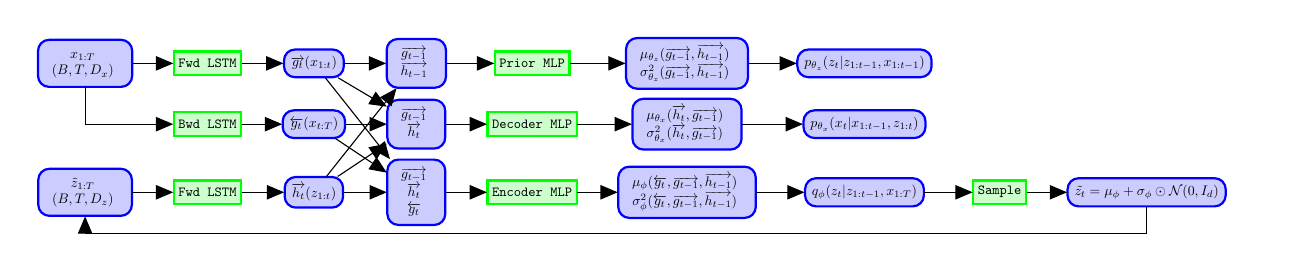
\begin{tikzpicture}[
    % format
    scale=0.50,
    every node/.style={scale=0.50},
    torch/.style={
        rectangle, 
        minimum size=6mm, 
        thick, 
        draw=green!100, 
        fill=green!20, 
        font=\ttfamily
        },
    math/.style={
        rectangle, 
        rounded corners, 
        thick, 
        draw=blue!100,
        fill=blue!20,
        align=center,
        anchor=center,
        inner sep=5pt
        },
    point/.style={
        circle,
        inner sep=0pt,
        minimum size=0pt,
        }
    ]
\matrix[row sep = 1mm, column sep=5mm] {
% row 1
\node[math] (xt) {
    $\begin{array}{c}
            x_{1:T} \\
            (B,T,D_x)
    \end{array}$
}; &
\node[torch] (fwd_lstm) {Fwd LSTM}; & 
\node[math] (gt) {$\overrightarrow{g_t}(x_{1:t})$}; &
\node[math] (g_t_1_et_h_t_1) {
    $\begin{array}{c}
        \overrightarrow{g_{t-1}} \\
        \overrightarrow{h_{t-1}}
    \end{array}$
}; &
\node[torch] (prior) {Prior MLP}; &
\node[math] (theta_z) {
    $\begin{array}{c}
            \mu_{\theta_z}(\overrightarrow{g_{t-1}}, \overrightarrow{h_{t-1}}) \\
            \sigma_{\theta_z}^2(\overrightarrow{g_{t-1}}, \overrightarrow{h_{t-1}})
    \end{array}$
}; &
\node[math] (p_theta_z) {$p_{\theta_z}(z_t \vert z_{1:t-1}, x_{1:t-1})$}; & \\
% row 2
\node[point] (coin3) {}; &
\node[torch] (bwd_lstm) {Bwd LSTM}; & 
\node[math] (gt2) {$\overleftarrow{g_t}(x_{t:T})$}; &
\node[math] (g_t_1_et_h_t) {
    $\begin{array}{c}
        \overrightarrow{g_{t-1}} \\
        \overrightarrow{h_{t}}
    \end{array}$
}; &
\node[torch] (decoder) {Decoder MLP}; &
\node[math] (theta_x) {
    $\begin{array}{c}
            \mu_{\theta_x}(\overrightarrow{h_t}, \overrightarrow{g_{t-1}}) \\
            \sigma_{\theta_x}^2(\overrightarrow{h_t}, \overrightarrow{g_{t-1}})
    \end{array}$
}; & 
\node[math] (p_theta_x) {$p_{\theta_x}(x_t \vert x_{1:t-1}, z_{1:t} )$}; & \\
% row 3
\node[math] (z_tilde) {
    $\begin{array}{c}
            \tilde{z}_{1:T} \\
            (B,T,D_z)
    \end{array}$
}; & 
\node[torch] (fwd_lstm2) {Fwd LSTM}; & 
\node[math] (ht) {$\overrightarrow{h_t}(z_{1:t})$}; &
\node[math] (g_t_1_et_h_t_1_et_g_t) {
    $\begin{array}{c}
        \overrightarrow{g_{t-1}} \\
        \overrightarrow{h_{t}} \\
        \overleftarrow{g_t}
    \end{array}$
}; &
\node[torch] (encoder) {Encoder MLP}; &
\node[math] (phi) {
    $\begin{array}{c}
            \mu_{\phi}(\overleftarrow{g_{t}}, \overrightarrow{g_{t-1}}, \overrightarrow{h_{t-1}}) \\
            \sigma_{\phi}^2(\overleftarrow{g_{t}}, \overrightarrow{g_{t-1}}, \overrightarrow{h_{t-1}})
    \end{array}$
}; & 
\node[math] (q_phi) {$q_{\phi}(z_t \vert z_{1:t-1}, x_{1:T} )$}; &
\node[torch] (sample) {Sample}; &
\node[math] (z_tilde_formula) {$\tilde{z_t} = \mu_{\phi} + \sigma_{\phi} \odot \mathcal{N}(0, I_d)$}; & \\
% row 4
\node[point] (coin1) {};
& & & & & & & &;
\node[point] (coin2) {}; & \\
};
\path   (xt) edge [->, thin] (fwd_lstm)
        (xt) edge[-, thin] (coin3)
        (fwd_lstm) edge [->, thin] (gt)
        (gt) edge[->, thin] (g_t_1_et_h_t_1)
        (gt) edge[->, thin] (g_t_1_et_h_t)
        (gt) edge[->, thin] (g_t_1_et_h_t_1_et_g_t)
        (g_t_1_et_h_t_1) edge[->, thin] (prior)
        (prior) edge[->, thin] (theta_z)
        (theta_z) edge[->, thin] (p_theta_z)
        (coin3) edge[->, thin] (bwd_lstm)
        (bwd_lstm) edge[->, thin] (gt2)
        (gt2) edge[->, thin] (g_t_1_et_h_t)
        (gt2) edge[->, thin] (g_t_1_et_h_t_1_et_g_t)
        (g_t_1_et_h_t) edge[->, thin] (decoder)
        (decoder) edge[->, thin] (theta_x)
        (theta_x) edge[->, thin] (p_theta_x)
        (z_tilde) edge[->, thin] (fwd_lstm2)
        (fwd_lstm2) edge[->, thin] (ht)
        (ht) edge[->, thin] (g_t_1_et_h_t_1_et_g_t)
        (ht) edge[->, thin] (g_t_1_et_h_t)
        (ht) edge[->, thin] (g_t_1_et_h_t_1)
        (g_t_1_et_h_t_1_et_g_t) edge[->, thin] (encoder)
        (encoder) edge[->, thin] (phi)
        (phi) edge[->, thin] (q_phi)
        (q_phi) edge[->, thin] (sample)
        (sample) edge[->, thin] (z_tilde_formula)
        (z_tilde_formula) edge[-, thin] (coin2)
        (coin2) edge[-, thin] (coin1)
        (coin1) edge[->, thin] (z_tilde);
\end{tikzpicture}


% LOSS

% --- Loss VRNN
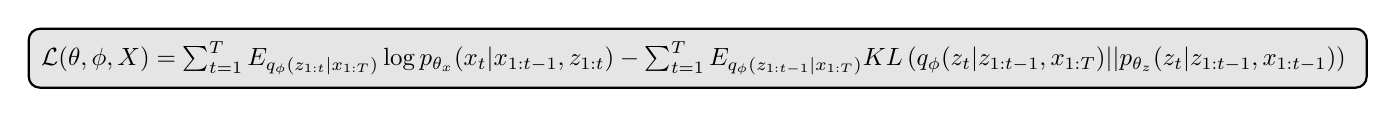
\begin{tikzpicture}[
    scale=0.90,
    every node/.style={scale=0.90},
    math/.style={
        rectangle, 
        % minimum height=1cm,
        % minimum width=2cm,
        rounded corners, 
        thick, 
        draw=black!100,
        fill=gray!20,
        align=center,
        anchor=center,
        inner sep=5pt
        },
    ]
    \node[math] {
        $\VLB = \sum_{t=1}^T  \E{q_{\phi}(z_{1:t} \vert x_{1:T})} \log{p_{\theta_x}(x_t \vert x_{1:t-1}, z_{1:t})} - \sum_{t=1}^T \E{q_{\phi}(z_{1:t-1} \vert x_{1:T})} \KL{q_{\phi}(z_t \vert z_{1:t-1}, x_{1:T})}{p_{\theta_z}(z_t \vert z_{1:t-1}, x_{1:t-1})}$
    };
\end{tikzpicture}

\end{frame}
\section{DVAE and Stochastic Differential Equations}\label{DVAEs and SDEs}

% ----- DEFINITION D'UN PROCESSUS STOCHASTIQUE

\begin{frame}{Stochastic calculus survival kit - Stochastic process}
    
\begin{definition}
    A \textbf{stochastic process} is defined as:
\begin{align}
    X &= (\Omega, \mathcal{F}, (\mathcal{F}_t)_{t \in T}, (X_t)_{t \in T}, \mathbb{P})
    %(\Omega, \mathcal{F}, (X_t)_{t \in T}, \mathbb{P}) \\
\end{align}
where:
    \begin{itemize}
        \item $\Omega$ is a set (universe of possibles).
        \item $\mathcal{F}$ is a $\sigma$-algebra of parts of $\Omega$
        \item $\mathbb{P}$ is a probability measure on $(\Omega, \mathcal{F})$
        \item $T \subset \mathbb{R}_+$ represents time
        \item $(\mathcal{F}_t)_{t \in T}$ is a \textbf{filtration}, ie an increasing family of sub-$\sigma$-algebras of $\mathcal{F}$ indexed by $t$ : $\forall 0 \leq s \leq t \in T$, $\mathcal{F}_s \subset \mathcal{F}_t \subset \mathcal{F}$.
        \item $(X_t)_{t \in T}$ is a family of RV defined on $(\Omega, \mathcal{F})$ with values in a measurable space $(E, \mathcal{E})$ or more simply $(E, \mathcal{B}(E))$ (set $E$ endowed with its Borelian $\sigma$-algebra).
        \item $(X_t)_{t \in T}$ is assumed \textbf{adapted to the filtration} $(\mathcal{F}_t)_{t \in T}$, meaning $\forall t \in T$, $X_t$ is $\mathcal{F}_t$-measurable
    \end{itemize}
\end{definition}

A filtration $\mathcal{F}_{t\geq 0}$ is often viewed and introduced as the \textit{set of information available at time $t$}. 

\end{frame}


% ---  BROWNIAN MOTION -------------


\begin{frame}{Stochastic calculus survival kit - Brownian motion}
\begin{definition}
A stochastic process $B = \brownian$ with values in $\mathbb{R}^d$ is called \textbf{Brownian motion} iff:
\begin{itemize}
    \item $B_0 = 0$ $\mathbb{P}$-a.s.
    \item $\forall 0 \leq s \leq t$, the random variable $B_t-B_s$ is independent from $\mathcal{F}_t$.
    \item $\forall 0 \leq s \leq t$, $B_t - B_s \sim \mathcal{N}(0,Q(t-s))$
    \item $B$ is continuous \footnote{or more exactly there exists a continuous version of $B$, see \cite{mouvement-brownien-calcul-ito}}
\end{itemize}
where the matrix $Q \in \mathbb{S}^{++}_d$ is called the \textbf{diffusion matrix}.
\end{definition}

% Meaning : the process $B$ starts from 0, its increments are independent from the past, its increments over disjoint time intervals are independent of each other, 
% its increments follow a centered normal law of variance equal to the length of the time interval multiplied by the diffusion matrix.
% NB : some authors choose the define the diffusion matrix (or scalar) outside of the Brownian motion.

A core result is that the quadratic variation of the Brownian motion over an interval $[s,t]$ (equiped
with a subdivison $\pi = \{s=t_0 < t_1 < ...< t_k <... < t_n=t\}$), and defined as the limit when $\vert \pi \vert \rightarrow 0$ 
of $V_{\pi}^{(2)} = \sum_{k=0}^{n-1} \vert f(t_{k+1})-f(t_k)\vert^{2}$, is:

\begin{align}
    &\underset{\vert \pi \vert \rightarrow 0}{\text{lim}}\,\, V_{\pi}^{(2)} = Q(t-s) \,\, \text{in} \,\, L^{2}
\end{align}

% Or, heuristically, 
% \begin{align}
%     \label{dB_square_is_dt}
%     \mathbb{E}(dB_t dB_t^T) = Q dt
% \end{align}
\end{frame}

% ------ STOCHASTIC INTEGRALS ----------------

\begin{frame}{Stochastic calculus survival kit - Stochastic Integrals}
    Ito then proceeds to define \textbf{stochastic integrals}, starting with elementary processes:

\begin{definition}
A stochastic process $X = (X_s)_{s \in [a,b]}$ is called \textbf{elementary} if there exists a subdivision $a = t_0 < t_1 < ... < t_n = b$ of $[a,b]$, such that:
\begin{align*}
    \forall t \in [a,b], \forall \omega \in \Omega, X_t(\omega) = \sum_{i=0}^{n-1} X_i(\omega) \textbf{1}_{[t_i, t_{i+1}[}(t)
\end{align*}
with $\forall i \in \{0,1,..,n-1\}, X_i$ is $\mathcal{F}_{t_i}$-measurable.

This means that, in each interval $[t_i, t_{i+1}[$, $X_t(\omega)$ is independent of $t$ and $X_t(\omega) = X_i(\omega)$.

We define $\mathcal{E}$ (resp. $\mathcal{E}_n, n>0$) the set of all elementary processes on $[a,b]$ (resp. the subset of the $X \in \mathcal{E}$) such that all $X_i$ have a finite moment $\mathbb{E}X_i <\infty$ (resp $\mathbb{E}(\vert X_i\vert^n) < \infty$).
\end{definition}
\end{frame}

\begin{frame}{Stochastic calculus survival kit - Stochastic Integrals 2}
\begin{definition}
Let $X \in \mathcal{E}$, ie
\begin{align*}
X_t(\omega) = \sum_{i=0}^{n-1} X_i(\omega) \textbf{1}_{[t_i, t_{i+1}[}(t)
\end{align*}
\textbf{The stochastic integral of $X$ is the real random variable} :
\begin{align*}
\int_a^b X_t dB_t := \sum_{i=0}^{n-1} X_i (B_{t_{i+1}} - B_{t_{i}})
\end{align*}
\end{definition}

The notion is then extended to other stochastic processes (in spaces of square integrable processes, see the annex).
\end{frame}


\begin{frame}{Stochastic calculus survival kit - Ito's process}
    \begin{definition}
    A process $X = (X_t)_{t \in [0, T]}$ is called a \textbf{Ito's process} if it can be written as:
    \begin{align}
        \label{ito sde definition}
        X_t &= X_0 + \int_{0}^{t}a_s ds + \int_{0}^{t} b_s dB_s \,\,\, \forall t \in [0,T]
    \end{align}
    where $a$ and $b$ are two stochastic processes such that the integrals exist (ie $a \in  \Lambda^1$ and 
    $b \in \Lambda^2$).\\
    Equivalently, we write $X_t$ as the soltuion to the \textbf{Stochastic Differential Equation}:
    \begin{align*}
        dX_t = a_t dt + b_t dB_t
    \end{align*}
    \end{definition}
\end{frame}

%
% ----- ITO FORMULA ------------------
%

\begin{frame}{Stochastic calculus survival kit - Ito's formula}
    
\begin{theorem}
An Itô's process remains an Itô's process when it is transformed by a deterministic function that is "smooth enough".

Let $X$ be a Itô's process on $[0,T]$ : $dX_t = a_tdt + b_t dB_t$.

Let $f : \mathbb{R} \times \mathbb{R} \rightarrow \mathbb{R}, (x,t) \mapsto f(x,t)$ be 
$\mathcal{C}^{2,1}$ : $\mathcal{C}^2$ in $x$, and $\mathcal{C}^1$ in $t$.

Then $(f(X_t,t))_{t \in [0,T]}$ is also an Itô's process and:
\begin{align}
    d\left( f(X_t,t) \right) = \frac{\partial f}{\partial t}(X_t,t) dt + \frac{\partial f}{\partial x}(X_t,t) dX_t + \frac{1}{2}\frac{\partial^2 f}{\partial x^2}(X_t,t)b_t^2 dt
\end{align}
The last term is Itô's complementary term.\\
In dimension $d > 1$:
\begin{align}
    d\left( f(X_t,t) \right) = \frac{\partial f}{\partial t}(X_t,t) dt + (\nabla f)^T (X_t,t) dX_t + \frac{1}{2}\text{Tr} \left( (\nabla \nabla^T f) dX_t dX_t^T \right)
\end{align}
\end{theorem}
\end{frame}

%
% --- SDE defintion
%

\begin{frame}{Definition of a Stochastic Differential Equation}
    \begin{definition}
            Let:
    \begin{itemize}
        \item $B$ be a Brownian motion $B_t \in \mathbb{R}^S$, of diffusion matrix $Q$
        \item $F$ be a deterministic function "drift" $F : \mathbb{R}^D \times \mathbb{R}\rightarrow \mathbb{R}^{D \times D}$
        \item $L$ be a deterministic function "dispersion" $L : \mathbb{R}^D \times \mathbb{R}\rightarrow \mathbb{R}^{D \times S}$ 
    \end{itemize}

    The \gls{sde} is:
    \begin{align}
        \label{generic_sde}
        dX_t &= F(X_t,t) dt + L(X_t,t) dB_t \\
        X_{t_0} &= X_0
    \end{align}
    where $X_0$ can be a scalar constant or a random variable.
    A stochastic process $X$ is said to be solution of \ref{generic_sde} if it verifies:
    \begin{align*}
        \forall t, \,\, X_t = X_0 + \int_{0}^{t} F(X_u, u)du + \int_{0}^{t} L(X_u,u) dB_u
    \end{align*}
    \end{definition}
\end{frame}

\begin{frame}{A solution to an SDE is a Markov Process}
\begin{itemize}
    \item As for \gls{ode}, a solution to \ref{generic_sde} might not exist. Also, results similar to Cauchy-Lipschitz 
exist for existence and unicity, based on assumptions on $F$ and $L$. 
    \item Intuitively, we can see that an "infinitesimal increment" of $X_t$ to $X_{t+\Delta_t}$ verifies :
$\Delta {X_t} \approx F(X_t, t) \Delta t + L(X_t,t) dB_t$. But $dB_t$ is a Brownian increment independent of $X_t$,
This suggests that $X_{t+ \Delta_t}$ depends on the past only by $X_t$. 
    \item In other words, $X_t \vert \mathcal{F}_s = X_t \vert X_s$ 
for any $0 < s < t$. ie : \textbf{the solution of a \gls{sde} is a Markov process}. (The formal proof is given in \cite{mouvement-brownien-calcul-ito}.)
\end{itemize}
\end{frame}

\begin{frame}{Transition Kernels}
    \begin{itemize}
        \item Formally, a Markov process is caracterized by its \textbf{transition kernels}. 
        \item That is, for any $s < t$, and any $A \in \mathcal{B}_{\mathbb{R}^{D}}$, a Markov process verifies 
$\mathbb{P}(X_t \in A \vert \mathcal{F}_s) = \mathbb{P}(X_t \in A \vert X_s)$.
        \item the transition kernels of $X$ are the applications $P_{s,t} : \mathbb{R}^{D} \times \mathcal{B}_{\mathbb{R}^{D}} \rightarrow [0,1]$, 
            such that for any $f : \mathbb{R}^{D} \rightarrow \mathbb{R}$ measurable and bounded, we have:
            \begin{align}
                P_{s,t}f(x) = \int_{{\mathbb{R}^{D}}} P_{s,t}(x,dy) f(y)
            \end{align}
        So $P_{s,t}$ actually is the probability measure of starting from $x$ at time $s$, and reach $y \in dy$ at time $t$.
    \end{itemize}
    
When the transition kernels have densities $p(x,t \vert y,s)$ (ie starting from $y$ at time $s$, and
reaching $x$ at time $t$), then a fundamental result is the \textbf{Fokker Plank Kolmogorov} equation 
(also known as forward Kolomogorov) :
\begin{align}
    \label{FPK}
    \frac{\partial p}{\partial y} &= \mathcal{A}^{*}p \\
    \mathcal{A}^{*}(\bullet) &= - \sum_{i=1}^{D} \frac{\partial}{\partial x_i} (F_i(x,t)(\bullet)) + \
        \frac{1}{2} \sum_{i,j=1}^{D} \frac{\partial^{2}}{\partial x_i \partial x_j} (L(x,t)QL(x,t)^{T}\vert_{i,j} (\bullet))
\end{align}
\end{frame}

\begin{frame}{Linear SDE}
    A particularly useful flavor of \gls{sde} is the linear \gls{sde}, that allows some close-form (or at least nicer) solutions:

    \begin{definition}
        With the same notations as \ref{generic_sde}:

        The linear \gls{sde} is:
        \begin{align}
            \label{linear_sde}
            dX_t &= F(t) X_t dt + L(t) dB_t \\
            X_{t_0} &= X_0 \sim \mathcal{N}(m_0, P_0)
        \end{align}
    \end{definition}
\end{frame}

\begin{frame}{Transition kernels for linear SDEs}
In this case, the transition kernels family can be characterized as:
\begin{align}
    \Psi &: \mathbb{R}^{2 } \rightarrow \mathbb{R}^{D} \\
    \frac{\partial \Psi (\tau, t)}{\partial \tau} &= F(\tau) \Psi(\tau, t) \\
    \frac{\partial \Psi (\tau, t)}{\partial t} &= - \Psi(\tau, t) F(t)  \\
    \Psi(\tau, t) &= \Psi(\tau, s) \Psi(s, t) \,\,\, (\text{Chapman-Kolmogorov}) \\
    \Psi(\tau, t) &= \Psi(t, \tau)^{-1} \\ 
    \Psi(t,t) &= I_d
\end{align}

% \begin{proposition}
\textbf{The solution to a linear SDE \ref{linear_sde} is a Gaussian Process}:
\begin{align}
    \label{solution_linear_sde}
    X_t &= \Psi(t,t_0) X_0 + \int_{t_0}^{t} \Psi(t, \tau) L(\tau) dB_{\tau} \\
    X_{t_0} &= X_0 \sim \mathcal{N}(m_0, P_0)
\end{align}
% \end{proposition}
\end{frame}

\begin{frame}{Beyond linear SDEs}
    \begin{itemize}
        \item In practice, we posit a stochastic process prior defined by a general \gls{sde}, and we have discrete-time measurements.
        \item Formally, the \gls{cd-ssm} is defined by:
            \begin{tcolorbox}[colback=blue!5!white,colframe=black!75!black,title=Continuous-Discrete State Space model]
                \begin{align}
                    dZ_t &= F(Z_t, t)dt + L(Z_t,t) dB_t \\
                    x_k &\sim p(x_k \vert z_{t_k})
                \end{align}
                where:
                \begin{itemize}
                    \item $Z_t \in \mathbb{R}^{D}$ is the \textit{state}, ie a stochastic process defining the latent variable.
                    \item $B_t \in \mathbb{R}^{S}$ is a Brownian motion with diffusion matrix $Q$.
                    \item $F \in \mathbb{R}^{D}$ and $L \in \mathbb{R}^{D \times S}$ are the usual drift and dispersion functions.
                    \item $x_k$ are the observations taken at \textbf{discrete times $(t_k)_{k=1,...,n}$}
                \end{itemize}
                NB : the observations are assumed to conditionnally independent of the state.
            \end{tcolorbox}
        % \item The \gls{gpvae} is a particular case of \gls{cd-ssm} with a linear \gls{sde}.
    \end{itemize}
\end{frame}

\begin{frame}{Filtering}
    \begin{itemize}
        \item \textbf{Filtering} is the problem of determining the posterior probability of the latent $Z_t$ given the 
discrete measurements, ie finding $p(Z_t \vert x_{1:k})$ with $t_k \leq t$. This corresponds to 
determining the generative transition probability $p_{\theta_z}(z_t \vert z_{1:t-1}, x_{1:t-1})$ in our 
\gls{dvae} setting.
        \item In general, close-form solutions can be derived when the latent variables \gls{sde} is linear. In continuous 
time, we get the \textbf{Kalman-Bucy} filter equations, which discretize in the well-known \textbf{Kalman filter}.
    \end{itemize}
\end{frame}

\begin{frame}{Filtering}
        \begin{tcolorbox}[colback=blue!5!white,colframe=black!75!black,title=Kalman-Bucy filter]
            \begin{align}
                dZ_t &= F(t)Z_t dt + L(t) dB_t \\
                dX_t &= H(t)X_t dt + d\eta_t
            \end{align}
            % \begin{itemize}
            %     \item $Z_t \in \mathbb{R}^{D}$ is the state/latent, $X_t \in \mathbb{R}^{M}$ is the observation/measurement.
            %     \item $B_t \in \mathbb{R}^{S}$ is a Brownian motion with diffusion matrix $Q$, $\eta_t \in \mathbb{R}^{S}$ is a BM with diffusion matrix $R$.
            %     \item $F \in \mathbb{R}^{D}$ drift, $L \in \mathbb{R}^{D \times S}$ dispersion, $H \in \mathbb{R}^{D \times M}$ observation model.
            % \end{itemize}
            NB : the observations are assumed to conditionnally independent of the state.
            Then the Bayesian filter (Kalman-Bucy) is:
            \begin{align}
                p(z_t \vert x_{<t}) &= \mathcal{N}(Z_t \vert m_t, P_t) \\
                K &= P H(t)^{T} R^{-1} \\
                dm &= F(t)m dt + K (dX_t - H(t) m dt) \\
                \frac{dP}{dt} &= F(t)P + P F(t)^{T} + L(t)QL(t)^{T} - KRK^{T}
            \end{align}
        \end{tcolorbox}
\end{frame}

\begin{frame}{Smoothing}
    \begin{itemize}
        \item \textbf{Smoothing} is the problem of determining the posterior probability of the latent $Z_t$ given 
all known observations, ie finding $p(Z_t \vert x_{1:T})$ for all $t \in [0,T]$. 
        \item This corresponds to determining the inference model $q_{\phi}(z_t \vert z_{1:t-1}, x_{1:T})$ in the \gls{dvae} setting.
        \item Discretizing the transition density in \gls{cd-ssm}, we have
            \begin{align}
                Z_{t_{k+1}} &\sim p(Z_{t_{k+1}} \vert Z_{t_k}) \\
                X_k &\sim p(X_k \vert Z_{t_k})
            \end{align}
    \end{itemize}
\end{frame}

\begin{frame}
            \begin{tcolorbox}[colback=blue!5!white,colframe=black!75!black,title=Bayesian smoother]
                \begin{align}
                    Z_{t_{k+1}} &\sim p(Z_{t_{k+1}} \vert Z_{t_k}) \\
                    X_k &\sim p(X_k \vert Z_{t_k})
                \end{align}
                The \textit{Bayesian smoother} is, for any $k < T$:
                \begin{align}
                    p(Z_{t_{k+1}} \vert X_{1:k}) &= \int p(Z_{t_{k+1}} \vert Z_{t_k}) p(Z_{t_k} \vert X_{1:k}) dZ_{t_k} \\
                    p(Z_{t_k} \vert X_{1:T}) &= p(Z_{t_{k}} \vert X_{1:k})\int \left(
                        \frac{
                            p(Z_{t_{k+1}} \vert Z_{t_k}) p(Z_{t_{k+1}} \vert X_{1:T})
                        }{
                            p(Z_{t_{k+1}} \vert X_{1:k}
                        }dZ_{t_{k+1}}
                    \right)
                \end{align}
                The backward recursion is started from the final step, where the filtering and smoothing densities 
                are the same : $p(Z_{t_T} \vert X_{1:T})$.
            \end{tcolorbox}
\end{frame}


\begin{frame}{GP-VAE with accomodating kernels : filtering/smoothing in $O(n)$}
    \begin{itemize}
        \item We wrap up here linking the filtering/smoothing theory of linear \gls{sde} with the \gls{gpvae} 
model of \cite{fortuin_gp-vae:_2020}.
        \item Using the formalization above, a \gls{gpvae} with Gaussian observation is basically:
            \begin{align}
                \label{gpvae gaussian observation}
                Z_t &\sim \mathcal{GP}(m(\bullet), k(\bullet, \bullet)) \\
                X_{t_k} &\sim \mathcal{N}(X_{t_k} \vert Z_{t_k}, \sigma^{2})
            \end{align}
        \item Computing the posterior distribution $p(Z_t \vert X_{t_1:t_T})$ is performing a Gaussian Process 
regression (see \cite{rasmussen_gaussian_2008}), which naively scales in $O(n^{3})$.
        \item However, if the Gaussian process can be written as a linear \gls{sde}:
            \begin{align}
                \label{gpvae linear sde form}
                dZ_t &= F(t)Z_t dt + L(t)dB_t \\
                X_{t_k} &\sim \mathcal{N}(X_{t_k} \vert Z_{t_k}, \sigma^{2})
            \end{align}
            then the Kalman filter and smoother apply, that scale in $O(n)$. 
    \end{itemize}
\end{frame}

\begin{frame}{Gaussian Processes as solutions of linear SDE}
    \begin{itemize}
        \item \textbf{Brownian motion} : solution to $dZ_t = dB_t$, \gls{gp} with kernel $k(t,t') = \text{min}(t,t')$ (see \ref{sec:brownian_motion_gaussian_and_markov})
        \item \textbf{Ornstein Uhlenbeck} : the O.U. process
            \begin{align}
                dZ_t &= - \frac{1}{l} Z_t dt + dB_t
            \end{align}
            where $dB_t$ has diffusion coefficient $\frac{2 \sigma^{2}}{l}$, is a \gls{gp} with kernel:
            \begin{align}
                k_{\text{exp}} &= \sigma^{2} \exp{(- \frac{\vert t-t' \vert}{l})}
            \end{align}
        \item \textbf{Matern} : the \gls{sde} representation with
            \begin{align}
                F = \begin{pmatrix}
                    0 & 1 \\
                    -\lambda^{2} & -2 \lambda 
                \end{pmatrix}, 
                L = \begin{pmatrix}
                    0 \\ 1
                \end{pmatrix}, 
                H &= \begin{pmatrix}
                    1 \\ 0
                \end{pmatrix}
            \end{align}
            is a \gls{gp} with the Matern kernel with $\nu = \frac{3}{2}$:
            \begin{align}
                k_{\text{Matern}} &= \sigma^{2} \left(
                    1 + \frac{\sqrt{3} \vert t-t' \vert}{l}
                \right) \exp{
                    \left(
                        -\frac{\sqrt{3} \vert t-t' \vert}{l}
                    \right)
                }
        \end{align}
        and $\lambda = \frac{\sqrt{3}}{l}$, diffusion is $q = 4\lambda^{3}\sigma^{2}$.
    \end{itemize}
\end{frame}


\begin{frame}{Some Gaussian Processes are NOT solutions to linear \gls{sde}}
    Conversely, the following kernels can not be used to derive an associated linear \gls{sde}:

\begin{itemize}
    \item \textbf{squared exponential} : the widely used
    \begin{align}
        k_{\text{se}}(t,t') &= \sigma^{2} \exp{\left(
            - \frac{\vert t-t' \vert^{2}}{2l^{2}}
        \right)}
    \end{align}
    \item \textbf{rational quadratic}:
    \begin{align}
        k_{\text{rq}}(t,t') &= \sigma^{2} \left(
            1 + \frac{\vert t-t' \vert^{2}}{2 \alpha l^{2}}
        \right)^{-\alpha}
    \end{align}
    with $\alpha > 0$.
\end{itemize}

In that latter case, one can use spectral decomposition (ie Mercer's theorem, see MVA kernel class \cite{mva_kernel_class}) 
to approximate the kernel function and determine an associated linear \gls{sde}.
\end{frame}
\section{Outro}\label{outro}

\begin{frame}{Outro}
    Conclusions
\end{frame}

\begin{frame}[allowframebreaks,noframenumbering]{References}
    \footnotesize
    \printbibliography[heading=none]
\end{frame}

% annexes

% \section{Annexes}\label{annexes}

\begin{frame}{Annexes}
    Annexes
\end{frame}

% \begin{frame}
%     \printglossary
% \end{frame}

\end{document}